\section{Human to Human Handover}
\label{sec:human}

In this section we describe the human-human experiments performed, the different objects, and the acquired data for analysis of handover motions. The section includes analysis of the handover motion in terms of velocity over the trajectory as well as velocity along time, followed by an overall discussion on the different types of handover motions. 

\subsection{Experimental Scenario}

The HHI dataset was gathered as a collaboration between 
École polytechnique fédérale de Lausanne (EPFL) and Karlsruher Institut für Technologie (KIT) \cite{starke_force_2019}. It involves two humans interacting with an object whether to grasp and handover to one another, or to manipulate and place it on a table. The focus of this work is solely on the handover motion. Figure \ref{fig:epfl_dataset} shows a frame of the handover trajectory of the different cups for each of the participants. The experiments includes data of 4 participants, all male, age between 25-35 years old, with a graduate academic background. The recorded data includes motion tracking markers from the OptiTrack system on the participant's wrist and on the cups, as well as data gloves from the CyberGlove system on the participant's hand (not used in this work).

    \begin{figure}
        \centering
        \begin{tabular}{@{}c@{}}
            \centering
            \includegraphics[width=0.225\textwidth,height=0.15\textheight]{Images/frame000023.png}
        \end{tabular}
        \begin{tabular}{@{}c@{}}
            \centering 
            \includegraphics[width=0.225\textwidth,height=0.15\textheight]{Images/frame000046.png}
        \end{tabular}
        \baselineskip
        \begin{tabular}{@{}c@{}}
            \centering 
            \includegraphics[width=0.225\textwidth,height=0.15\textheight]{Images/frame000117.png}
        \end{tabular}
        \begin{tabular}{@{}c@{}}
            \centering 
            \includegraphics[width=0.225\textwidth,height=0.15\textheight]{Images/frame000144.png}
        \end{tabular}
        \caption{The 4 participants with the 4 cups}
        \label{fig:epfl_dataset}
    \end{figure}
    
The handovers of the cups happen under two distinct situations: (i) an empty cup, and (ii) a cup 90\% filled with water. Each participant hands-over the different cups to a second participant (also present in the dataset but not analysed during the handover), and each cup is manipulated for both conditions. The cups relevant for this work are the red plastic cup (bottom-left), the transparent plastic cup (top-left), the champagne plastic cup (top-right), and the opaque wine glass (bottom-right). The handover trajectory is recorded at 120 Hz, taking on average 1-3 seconds, corresponding to 100-300 data points. A total of 100 handover trajectories are segmented for all the participants with the 4 cups in the two conditions.

The purpose of performing these experiments has to do with the lack of available datasets on human manipulating cups with different internal properties, such as material composition, shape, weight, and with varying conditions such as liquid level. There is also not been, to our knowledge, an extensive analysis on the impact of those varying properties on the kinematic control approaches of humans and possible applications to robots. 

\subsection{Handover Motion Analysis}

    \begin{figure}
        \centering
        \begin{tabular}{@{}c@{}}
            \centering
            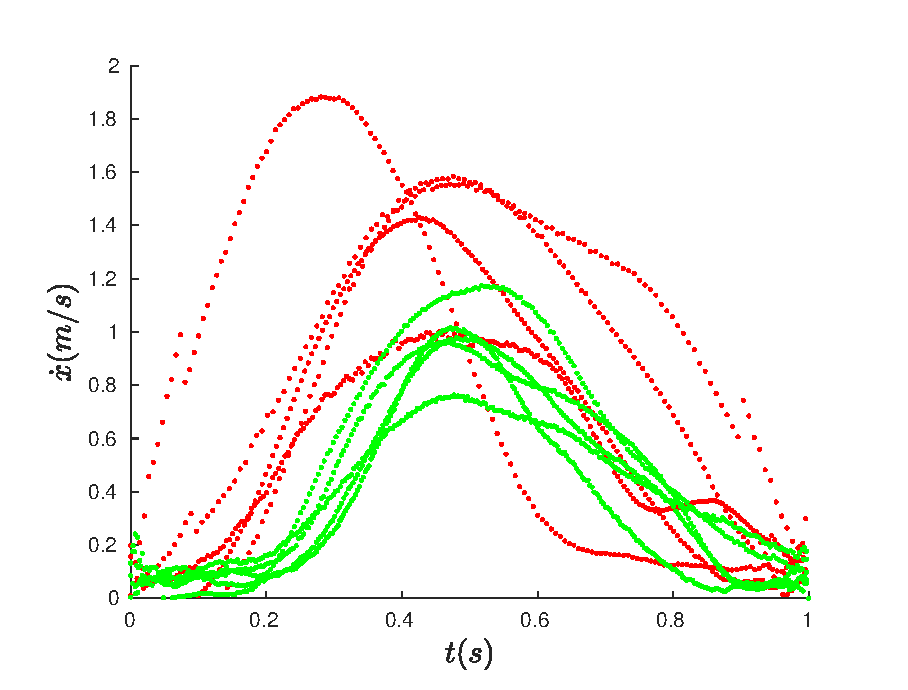
\includegraphics[width=0.48\textwidth,height=0.25\textheight]{Images/vel_distance_plot.eps}
        \end{tabular}
        \baselineskip
        \begin{tabular}{@{}c@{}}
            \centering 
            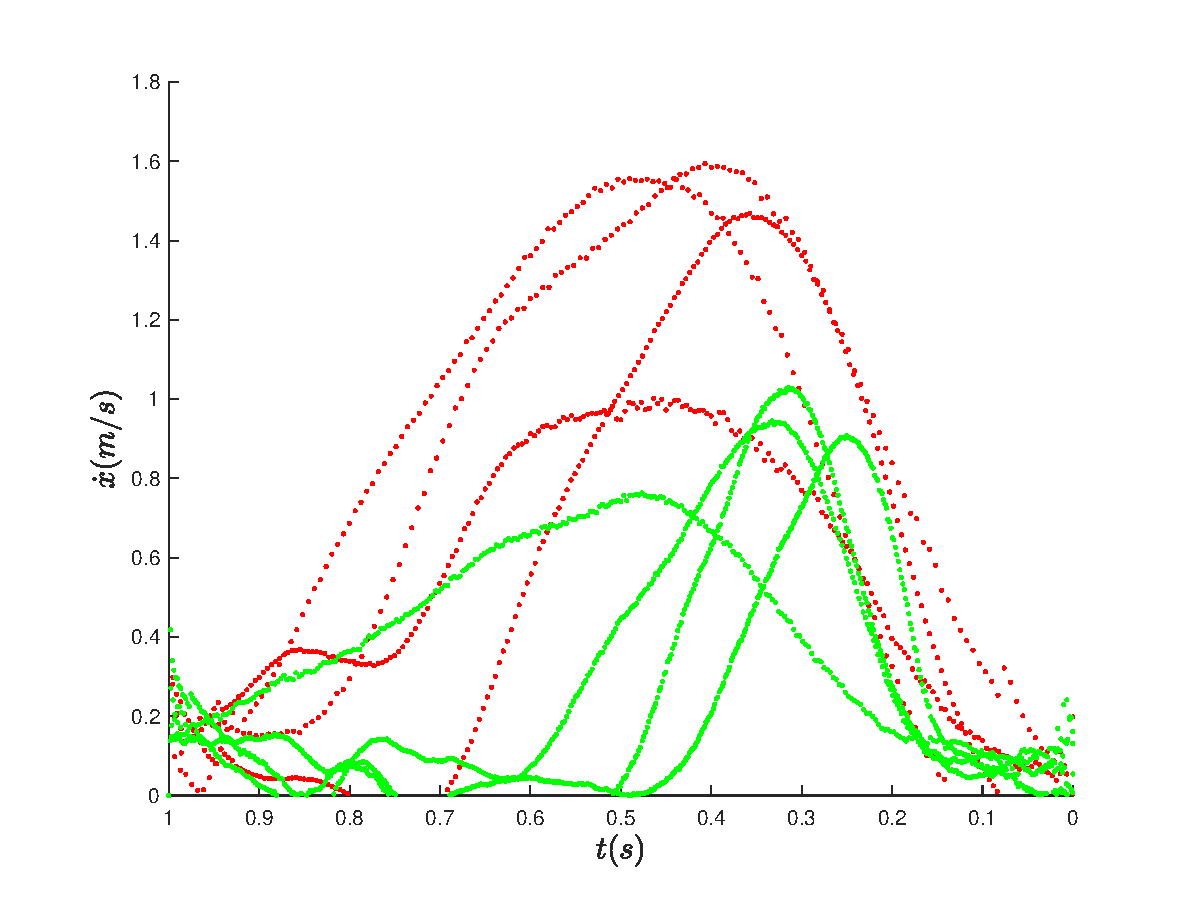
\includegraphics[width=0.48\textwidth,height=0.25\textheight]{Images/vel_time_plot.eps}
        \end{tabular}
        \caption{Sample of the dataset. Velocity/distance (top) and velocity/time (bottom).}
        \label{fig:vel_distance_time}
    \end{figure}

- analysis the data distance/velocity (inverse time of flight)

- analysis the data time/velocity

- mention Tamara Flash's work on minimum-jerk model (empirical analysis on point-to-point human motion) and state that the figure 3 gives the same minimum-jerk movement as stated by Flash

- mention that in the results we present two other datasets (QMUL, IST)

\subsection{Discussion}

- resume what you see from the data analysis of the human wrist

